\documentclass[border=10pt,varwidth]{standalone}
\usepackage{tikz}
\usetikzlibrary{shapes,arrows,shapes.multipart, positioning}

\begin{document}

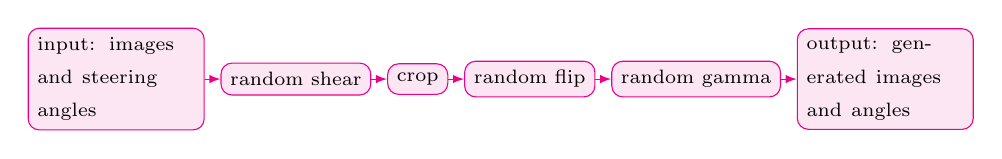
\begin{tikzpicture}
    \tikzset{
        node/.style = {rectangle, draw=magenta,  fill=magenta!10, thin, rounded corners},
        line/.style = {draw=magenta, thin, -latex},
        output/.style = {circle, draw=magenta,  fill=magenta!10, thin},
    }
    
    \node[node](input)[text width=2cm]{\scriptsize input: images and steering angles};
    
    \node[node](shear)[right = 0.2cm of input]{\scriptsize random shear};
    
    \node[node](crop)[right = 0.2cm of shear]{\scriptsize crop};
    
    \node[node](flip)[right = 0.2cm of crop]{\scriptsize random flip};   
    
    \node[node](gamma)[right = 0.2cm of flip]{\scriptsize random gamma}; 
    
    \node[node](resize)[right = 0.2cm of gamma, text width=2cm]{\scriptsize output: generated images and angles};
    
    \path [line] (input) -- (shear);
    \path [line] (shear) -- (crop);
    \path [line] (crop) -- (flip);
    \path [line] (flip) -- (gamma);
    \path [line] (gamma) -- (resize);
    

\end{tikzpicture}

\end{document}
